\documentclass[14pt]{extbook}
\usepackage{multicol, enumerate, enumitem, hyperref, color, soul, setspace, parskip, fancyhdr} %General Packages
\usepackage{amssymb, amsthm, amsmath, latexsym, units, mathtools} %Math Packages
\everymath{\displaystyle} %All math in Display Style
% Packages with additional options
\usepackage[headsep=0.5cm,headheight=12pt, left=1 in,right= 1 in,top= 1 in,bottom= 1 in]{geometry}
\usepackage[usenames,dvipsnames]{xcolor}
\usepackage{dashrule}  % Package to use the command below to create lines between items
\newcommand{\litem}[1]{\item#1\hspace*{-1cm}\rule{\textwidth}{0.4pt}}
\pagestyle{fancy}
\lhead{Module2}
\chead{}
\rhead{Version A}
\lfoot{3163-1865}
\cfoot{}
\rfoot{test}
\begin{document}

\begin{enumerate}
\litem{
Write the equation of the line in the graph below in Standard form $Ax+By=C$. Then, choose the intervals that contain $A, B, \text{ and } C$.
\begin{center}
    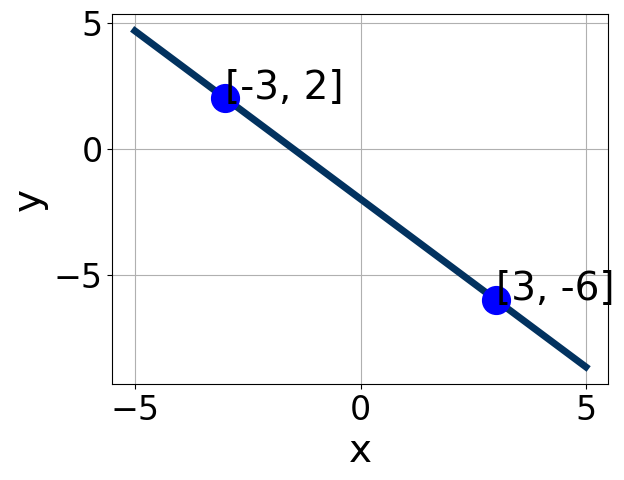
\includegraphics[width=0.5\textwidth]{../Figures/linearGraphToStandardA.png}
\end{center}
\begin{enumerate}[label=\Alph*.]
\item \( A \in [-0.1, 3.2], \hspace{3mm} B \in [-2.3, -0.1], \text{ and } \hspace{3mm} C \in [-1.1, 2.6] \)
\item \( A \in [3.6, 4.5], \hspace{3mm} B \in [-4.5, -1.3], \text{ and } \hspace{3mm} C \in [3.8, 8.2] \)
\item \( A \in [-0.1, 3.2], \hspace{3mm} B \in [0.3, 1.6], \text{ and } \hspace{3mm} C \in [-3.9, -0.8] \)
\item \( A \in [-4.2, -3.2], \hspace{3mm} B \in [-4.5, -1.3], \text{ and } \hspace{3mm} C \in [3.8, 8.2] \)
\item \( A \in [3.6, 4.5], \hspace{3mm} B \in [1.6, 4.2], \text{ and } \hspace{3mm} C \in [-8.6, -5.6] \)

\end{enumerate} }
\litem{
First, find the equation of the line containing the two points below. Then, write the equation as $ y=mx+b $ and choose the intervals that contain $m$ and $b$.\[ (-3, 2) \text{ and } (-8, -5) \]\begin{enumerate}[label=\Alph*.]
\item \( m \in [-5.4, -0.4] \hspace*{3mm} b \in [-16.77, -16.03] \)
\item \( m \in [1.4, 7.4] \hspace*{3mm} b \in [6.07, 7.44] \)
\item \( m \in [1.4, 7.4] \hspace*{3mm} b \in [-6.52, -5.39] \)
\item \( m \in [1.4, 7.4] \hspace*{3mm} b \in [2.99, 4.47] \)
\item \( m \in [1.4, 7.4] \hspace*{3mm} b \in [4.84, 5.55] \)

\end{enumerate} }
\litem{
Solve the equation below. Then, choose the interval that contains the solution.\[ -15(-16x -4) = -2(10x + 17) \]\begin{enumerate}[label=\Alph*.]
\item \( x \in [-0.12, -0.11] \)
\item \( x \in [-0.37, -0.36] \)
\item \( x \in [-0.1, -0.09] \)
\item \( x \in [0.09, 0.12] \)
\item \( \text{There are no real solutions.} \)

\end{enumerate} }
\litem{
Find the equation of the line described below. Write the linear equation as $ y=mx+b $ and choose the intervals that contain $m$ and $b$.\[ \text{Perpendicular to } 8 x + 5 y = 12 \text{ and passing through the point } (3, -9). \]\begin{enumerate}[label=\Alph*.]
\item \( m \in [-0.6, 1.2] \hspace*{3mm} b \in [-11.88, -9.88] \)
\item \( m \in [-0.6, 1.2] \hspace*{3mm} b \in [-15, -11] \)
\item \( m \in [-1.1, -0.3] \hspace*{3mm} b \in [-8.12, -4.12] \)
\item \( m \in [0.8, 3.4] \hspace*{3mm} b \in [-11.88, -9.88] \)
\item \( m \in [-0.6, 1.2] \hspace*{3mm} b \in [5.88, 15.88] \)

\end{enumerate} }
\litem{
Write the equation of the line in the graph below in Standard form $Ax+By=C$. Then, choose the intervals that contain $A, B, \text{ and } C$.
\begin{center}
    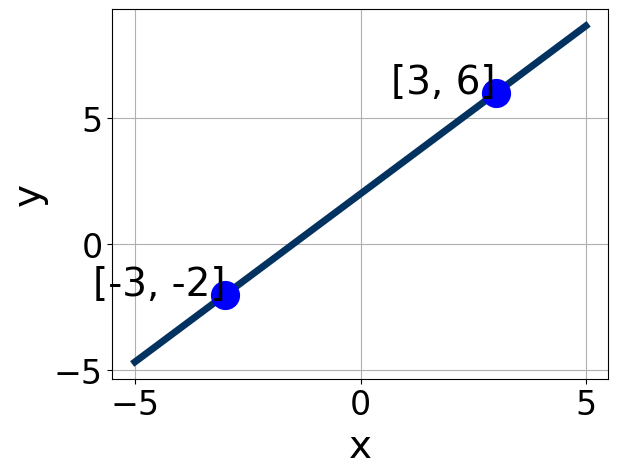
\includegraphics[width=0.5\textwidth]{../Figures/linearGraphToStandardCopyA.png}
\end{center}
\begin{enumerate}[label=\Alph*.]
\item \( A \in [-8, -4], \hspace{3mm} B \in [-5.9, -2.7], \text{ and } \hspace{3mm} C \in [-1, 5] \)
\item \( A \in [3, 8], \hspace{3mm} B \in [2, 5.3], \text{ and } \hspace{3mm} C \in [-1, 5] \)
\item \( A \in [-4.75, 3.25], \hspace{3mm} B \in [-2.5, 0.8], \text{ and } \hspace{3mm} C \in [-1, 5] \)
\item \( A \in [-4.75, 3.25], \hspace{3mm} B \in [0, 3], \text{ and } \hspace{3mm} C \in [-1, 5] \)
\item \( A \in [3, 8], \hspace{3mm} B \in [-5.9, -2.7], \text{ and } \hspace{3mm} C \in [-1, 5] \)

\end{enumerate} }
\litem{
Find the equation of the line described below. Write the linear equation as $ y=mx+b $ and choose the intervals that contain $m$ and $b$.\[ \text{Parallel to } 5 x - 7 y = 4 \text{ and passing through the point } (5, 7). \]\begin{enumerate}[label=\Alph*.]
\item \( m \in [-1.21, -0.18] \hspace*{3mm} b \in [9.3, 12] \)
\item \( m \in [0.25, 0.9] \hspace*{3mm} b \in [-4, -2.3] \)
\item \( m \in [0.25, 0.9] \hspace*{3mm} b \in [1.3, 2.1] \)
\item \( m \in [1.03, 2.43] \hspace*{3mm} b \in [3.1, 4.4] \)
\item \( m \in [0.25, 0.9] \hspace*{3mm} b \in [3.1, 4.4] \)

\end{enumerate} }
\litem{
First, find the equation of the line containing the two points below. Then, write the equation as $ y=mx+b $ and choose the intervals that contain $m$ and $b$.\[ (4, -6) \text{ and } (-6, -9) \]\begin{enumerate}[label=\Alph*.]
\item \( m \in [0.02, 0.78] \hspace*{3mm} b \in [-4.01, -2.89] \)
\item \( m \in [0.02, 0.78] \hspace*{3mm} b \in [-10.37, -9.02] \)
\item \( m \in [0.02, 0.78] \hspace*{3mm} b \in [6.78, 8.86] \)
\item \( m \in [-0.36, 0.17] \hspace*{3mm} b \in [-10.84, -10.72] \)
\item \( m \in [0.02, 0.78] \hspace*{3mm} b \in [-7.57, -5.34] \)

\end{enumerate} }
\litem{
Solve the linear equation below. Then, choose the interval that contains the solution.\[ \frac{7x + 3}{7} - \frac{-4x -8}{3} = \frac{5x -3}{8} \]\begin{enumerate}[label=\Alph*.]
\item \( x \in [-0.9, 0] \)
\item \( x \in [-2.5, -1.4] \)
\item \( x \in [-8.7, -7.3] \)
\item \( x \in [-0.5, 1.8] \)
\item \( \text{There are no real solutions.} \)

\end{enumerate} }
\litem{
Solve the linear equation below. Then, choose the interval that contains the solution.\[ \frac{-9x -7}{7} - \frac{-4x + 9}{3} = \frac{-9x + 6}{4} \]\begin{enumerate}[label=\Alph*.]
\item \( x \in [0.7, 1.9] \)
\item \( x \in [9.3, 10.2] \)
\item \( x \in [2.3, 4.6] \)
\item \( x \in [-2, 0] \)
\item \( \text{There are no real solutions.} \)

\end{enumerate} }
\litem{
Solve the equation below. Then, choose the interval that contains the solution.\[ -18(15x + 9) = -2(16x -10) \]\begin{enumerate}[label=\Alph*.]
\item \( x \in [-0.88, -0.64] \)
\item \( x \in [-0.51, -0.43] \)
\item \( x \in [0.5, 0.85] \)
\item \( x \in [-0.68, -0.48] \)
\item \( \text{There are no real solutions.} \)

\end{enumerate} }
\end{enumerate}

\end{document}